\section{Empirical Corroboration}\label{sec:empirical}

We do not claim accelerator-beam measurements. The empirical content
of v1 has two parts: a re-reading of the FTRFS v1 software validation
dataset~\cite{desbrieres2026ftrfs} through the calculus, and a
projected recovery surface derived from canonical SEU cross-section
data.

\subsection{Re-Reading the FTRFS v1 Dataset}

\Cref{tab:ftrfs-recovery} re-reads the four reproducible bench
metrics of FTRFS v1 (Sec.~VII of~\cite{desbrieres2026ftrfs}) through
the recovery-calculus lens. For each metric, we ask: which steps
of~\(\mathcal{G}\) does this metric exercise? The answer determines
whether a regression on the metric would be evidence of a
recovery-calculus violation or merely of a throughput change.

\begin{table}[ht]
\centering\small
\caption{Recovery-calculus interpretation of FTRFS v1 metrics. The
``Steps reachable'' column lists the steps of~\(\mathcal{G}\) that
the metric \emph{would} reach if its hot-path syndromes were non-zero;
on the consistent-state hot path actually exercised by the FTRFS v1
bench, all four metrics terminate at step~1. The ``Invariants'' column
lists the invariants the reachable steps would touch.
Metric M3 (deletion bench) is omitted from the FTRFS v1 evaluation
in its current revision and is therefore not analysed here.}
\label{tab:ftrfs-recovery}
\begin{tabularx}{\columnwidth}{@{}l X l@{}}
\toprule
\textbf{Metric} & \textbf{Steps reachable} & \textbf{Invariants} \\
\midrule
M1 (write+fsync) & 1; potentially 4, 6 (coherence + journal) & I3, I4 \\
M2 (read cold)   & 1 (syndrome check)                        & I4 \\
M4 (stat bulk)   & 1 (syndrome on inode)                     & I4 \\
M5 (small write) & 1; potentially 4, 6 on bitmap + SB        & I3, I4 \\
\bottomrule
\end{tabularx}
\end{table}

The reading shows that the RS-correction step (step~2 of
\cref{def:G}) is never triggered on the consistent-state hot path
exercised by the FTRFS v1 bench: all four metrics terminate at
step~1, where syndromes are zero. M1 and M5 would reach steps~4
and~6 only if a correction had been issued upstream; neither metric
forces that condition. That is the right behavior for a throughput
bench, but it means the v1 dataset does not constrain the recovery
operator's worst-case behavior. A BEAMFS bench will need an explicit
fault-injection metric (M6: ``corrupt-then-mount'') that exercises
step~2--6 of~\(\mathcal{G}\). That metric is reserved for v2 of this report,
when fault-injection results from the FTRFS Phase~E campaign
(under development) will be available in publishable form.

\subsection{Projected Recovery Surface}

\Cref{fig:recovery-surface} shows the projected probability of
successful RS recovery as a function of two physical parameters:
the linear energy transfer (LET) of the incident particle and the
particle fluence over a representative exposure window. The surface
is computed from the canonical Petersen figure-of-merit
formulation~\cite{petersen1996} with the cross-section curves
of~\cref{fig:see-cross-section}, integrated over a typical
RS(255,239) shortened code with 8-symbol correction capacity per
subblock.

\begin{figure}[t]
\centering
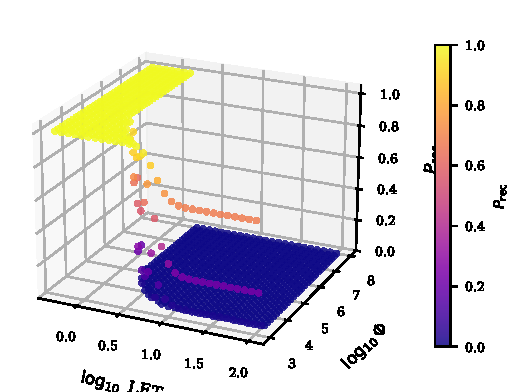
\includegraphics[width=\columnwidth]{figures/fig3.pdf}
\caption{Projected probability of successful Reed--Solomon recovery,
\(P_{\mathrm{rec}}(\mathrm{LET},\Phi)\), for an RS(255,239) shortened
code with 8-symbol correction capacity per subblock. Computed
analytically from canonical cross-section
data~\cite{petersen1996,baumann2005}; \emph{not} measured. The
plateau at \(P\approx 1\) is the Family-A regime where isolated SEU
events are well within RS capacity; the descent at high LET and
high~\(\Phi\) is the Family-B regime where MBU events saturate the
RS budget. Colour scale is plasma-like for print-monochrome
readability.}
\label{fig:recovery-surface}
\end{figure}
\FloatBarrier

The surface shows the expected qualitative structure: a wide plateau
at \(P \approx 1\) for low LET and low fluence (Family~A regime,
isolated SEU well within RS capacity), a transition zone where MBU
events begin to saturate the RS budget, and a low-\(P\) region where
the operator falls back to fail-closed (Family~B regime). The
transition is sharp by design: it corresponds to the Reed--Solomon
hard limit at 8 symbol errors per subblock, and the operator is
constructed to identify the transition cleanly rather than to
degrade gracefully through it.

\begin{remark}
A reviewer will object that this surface is computed from a model,
not measured. We agree, and the figure caption states this
explicitly. Measurement requires beam time: the present report is
the dossier from which beam-time at facilities such as
RADEF~(Jyv\"askyl\"a), GANIL, TRIUMF, Brookhaven NSRL or the ESA
REDLAB would be requested. The figure's purpose is to fix the
\emph{shape} of the expected dependency, against which future
measurements will be compared.
\end{remark}
